In cui si descrive la progettazione del software a un più basso livello: scelte progettuali, tecnologie e linguaggi adottati.

\section{Greenbone OpenVAS}
Come backend di scansione per il sistema, inizialmente si è optato per interfacciarsi a \textbf{Greenbone OpenVAS}.

\section{Base dati}
Il framework di Greenbone già include un suo database interno per la gestione degli utenti e dei ruoli associati ad essi, così come per le scansioni, i risultati e la reportistica. Inoltre, gran parte della logica di business rilevante è già definita e può essere personalizzata con un sistema di permessi abbastanza preciso e granulare, rendendo possibile adattarla facilmente ai nostri scopi.

Per questo motivo, si è deciso di non introdurre ridondanza e complessità con un ulteriore database, preferendo invece rimanere aderenti alla base di dati esistente, effettivamente sposando in tutto e per tutto la struttura dei dati proposta da Greenbone.

\subsection{Schema dei dati originale}
Lo schema dei dati proposto da Greenbone è strutturato come illustrato in figura \ref{er-crow}\footnote{Si noti che il diagramma ER qui realizzato rappresenta solamente le entità d'interesse considerate per il progetto: il reale database contiene uno schema più esteso e maggiormente interconnesso.}. In particolare:
\begin{itemize}
    \item Una \textbf{Task} rappresenta una scansione predisposta e configurata da un utente (\textbf{User}).
    \item Un utente appartiene ad uno o più ruoli (\textbf{Role}) (nel nostro caso specifico apparterrà sempre a uno ed un solo ruolo). Ogni ruolo inoltre può possedere dei permessi (\textbf{Permission}).
    \item Allo stesso modo, un utente appartiene ad uno o più gruppi (\textbf{Group}) (nel nostro caso specifico l'utente apparterrà al massimo sempre ad un gruppo). Anche i gruppi sono associati a dei permessi.
    \item I permessi sono espressi da un \emph{soggetto} su una \emph{risorsa}. Sia \emph{risorsa} che \emph{soggetto} rappresentano una qualunque entità del sistema, di qualunque tipo.
    \item Ad ogni risorsa possono essere associati uno o più \textbf{Tag} in forma di coppie nome valore. Nel nostro caso useremo questi tag per esprimere la quota dell'utente e pertanto saranno usati solo come decorazione ulteriore dell'entità utente.
    \item Un task è associato a delle preferenze di scansione (\textbf{Preference}). Queste preferenze sono espresse in XML e rappresentano dei dettagli di funzionamento, tra cui soprattutto la \emph{retention policy} dei rapporti generati.
    \item Ogni task è associato a una configurazione di scansione (\textbf{Config}). Questa prescrive in buona sostanza quali VT / NVT vengono eseguiti dalla scansione. Si noti che Greenbone esternamente distingue tra due tipi di configurazione di scansione:
    \begin{itemize}
        \item \emph{Scan config}: ovvero una semplice configurazione definita da un utente umano.
        \item \emph{Policy}: ovvero una scansione prescritta a norma di legge o in ottemperanza a qualche specifico standard. Queste ovviamente andrebbero lasciate così come fornite dal feed.
    \end{itemize}
    Questa distinzione internamente non è gestita con una separazione in entità distinte, come si può vedere dallo schema (allo stesso modo il progetto realizzato non fa distinzioni tra le due tipologie di configurazioni, internamente).
    \item Ogni scansione viene eseguita su un bersaglio specifico (\textbf{Target}). Un bersaglio di Greenbone OpenVAS specifica uno o più nodi di rete da scansionare, dettagliando anche eventuali credenziali di rete da usare per simulare un attacco di tipo \emph{white box}\footnote{In un attacco / test di tipo \emph{white box} l'attaccante è a disposizione di conoscenza rilevante e approfondita circa l'infrastruttura bersaglio. In un test \emph{black box} invece non viene fornito nessun aiuto / informazione, mentre in un \emph{gray box} vi è una via di mezzo, rappresentando di fatto la tipologia d'attacco più comune.} e le porte da considerare nella scansione.
    \begin{itemize}
        \item Le porte sono definite tramite un'entità \textbf{Portlist} associata. Questa internamente definisce le singole porte in modo efficiente tramite dei \emph{range} divisi per tipo (UDP o TCP).
    \end{itemize}
    \item Un task è eseguito da uno \textbf{Scanner}. In pratica questo è quasi sempre OpenVAS, ma Greenbone mette a disposizione anche uno scanner fittizio detto \textbf{CVE}, già dettagliato in \ref{cve}.
    \item Un task può essere associato anche ad una \textbf{Schedule}, che ne definisce un'eventuale esecuzione futura / ritardata e/o periodica / ricorrente. A basso livello la schedule è espressa tramite standard \textbf{iCalendar}.
    \item Un task contiene informazioni relative alla sua esecuzione, come il suo stato (in pausa, in esecuzione, in coda, fallita per errore, ecc.) e la percentuale di completamento.
    \item Infine, un task genera uno o più \textbf{Report}. Questi recano informazioni sul periodo temporale a cui sono riferiti e sul numero delle vulnerabilità trovate, nonché la loro severità. Le vulnerabilità si dividono in:
    \begin{itemize}
        \item \textbf{Falsi positivi}: vulnerabilità rilevate dal processo di scansione, ma che lo scanner è riuscito ad identificare autonomamente come falsi positivi.
        \item \textbf{Log}: spesso non sono vere e proprie vulnerabilità, ma semplici informazioni sul sistema di utilità quasi nulla. Alcune di queste sono solitamente disabilitate dagli amministratori di OpenVAS poiché inutilmente paranoiche.
        \item \textbf{Info}: vulnerabilità di basso livello, spesso che forniscono solo informazioni sul sistema, di utilità non nulla.
        \item \textbf{Warning}: vulnerabilità di medio livello, come vecchi standard crittografici ancora in uso, Denial of Service, ecc.
        \item \textbf{Hole / High / Critical}: vulnerabilità o problematiche ad alto livello di rischio e danno potenziale, come RCE, Privilege Escalation, EOL, ecc.
    \end{itemize}
    \item Un rapporto organizza quanto trovato in ``risultati'' (\textbf{Result}). Queste entità contengono metadati che descrivono testualmente la vulnerabilità, l'eventuale soluzione e forniscono gli riferimenti a CVE, CVSS e CPE relativi.
    \item Inoltre, l'esecuzione di un task rivela tutta una serie di \textbf{Asset} che vengono scoperti e inventariati durante la realizzazione del rapporto. Questi sono principalmente:
    \begin{itemize}
        \item \textbf{Host}, ovvero macchine fisiche o virtuali (questo comportamento può essere personalizzato come opzione dello scanner).
        \item Sistemi operativi (\textbf{OS}), con vari gradi di precisione nel loro processo di \emph{fingerprinting}.
    \end{itemize}
\end{itemize}

\begin{figure}
    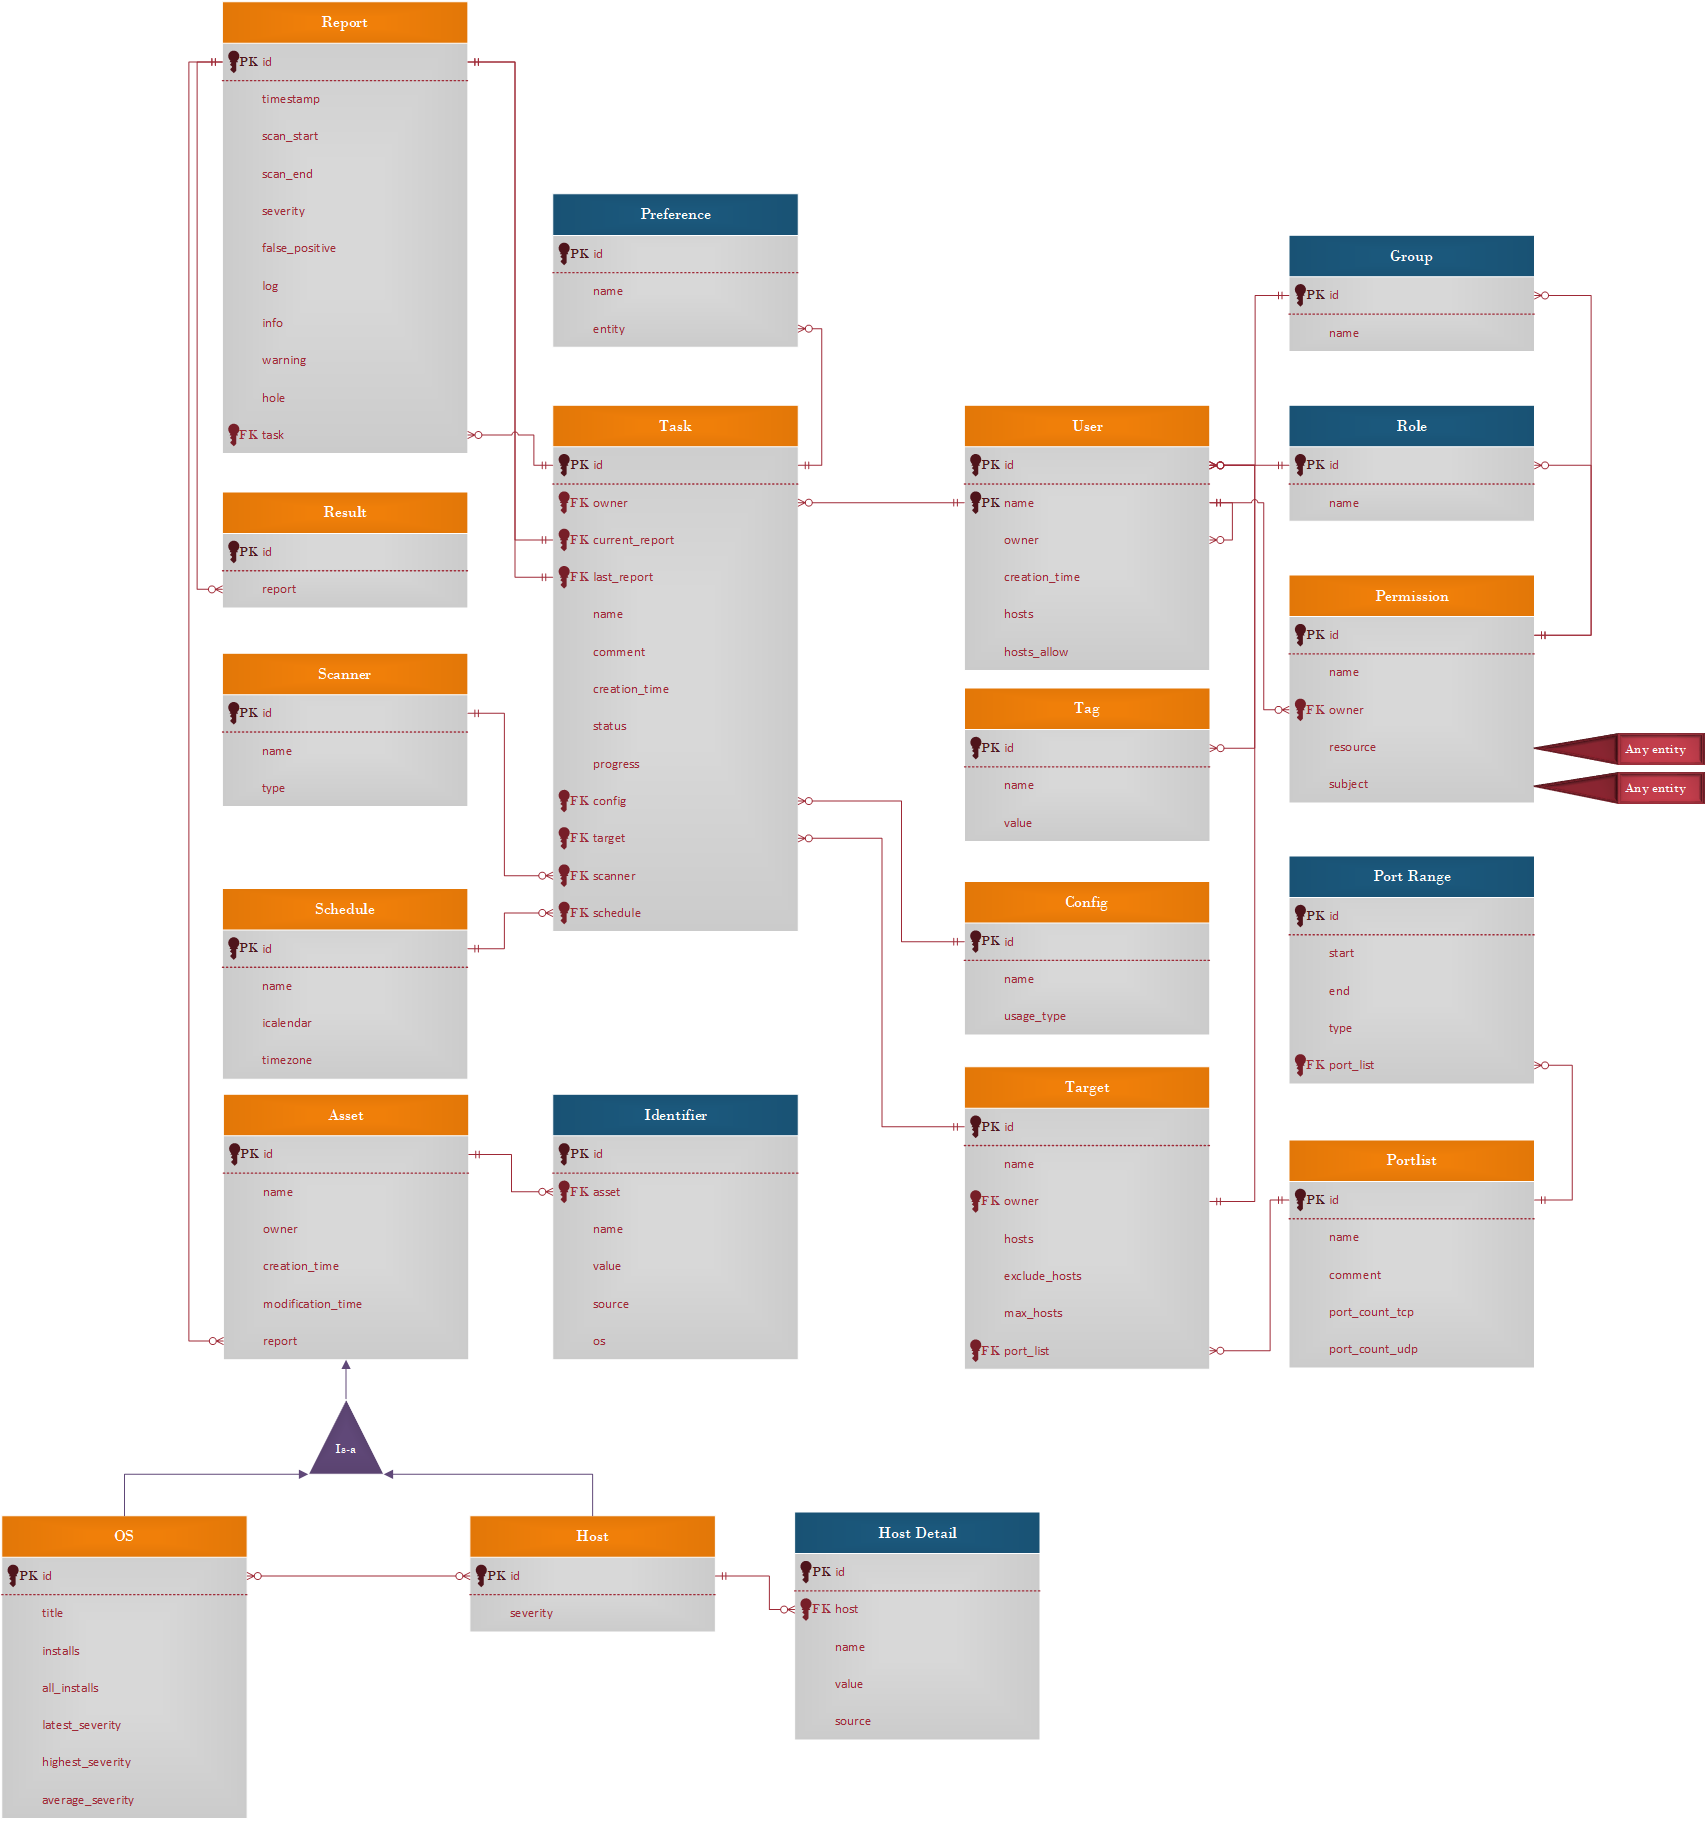
\includegraphics[width=\textwidth]{img/er_crow.png}
    \caption{Schema dei dati d'interesse di GVM}
    \label{er-crow}
\end{figure}

\section{Gerarchia degli utenti}
Si è scelto per la gerarchia a tre livelli \ref{3-level}, lasciando la gerarchia a quattro livelli \ref{4-level} come futuro sviluppo, essendo questa una semplice estensione della prima possibilità.